\section{Flusso di radiazione}
Energia del flusso: considerando un elemento di area $dA$ esposto alla radiazione per un tempo $dt$, la quantità di energia che attraversa l'elemento sarà proporzionale a $dAdt$. Scriviamo
\begin{equation}
    dE=F\,dA\,dt,
    \label{001}
\end{equation}
con $F$ flusso di energis, misurato in $\um{erg}\um{s}^{-1}\um{cm}^-2$.\\
Una sorgente di radiazione si dice isotropa quando emette energia in ugual modo in tutte le direzioni.
\begin{wrapfigure}{r}{0pt}
    \centering
    \resizebox{.3\columnwidth}{!}{%
        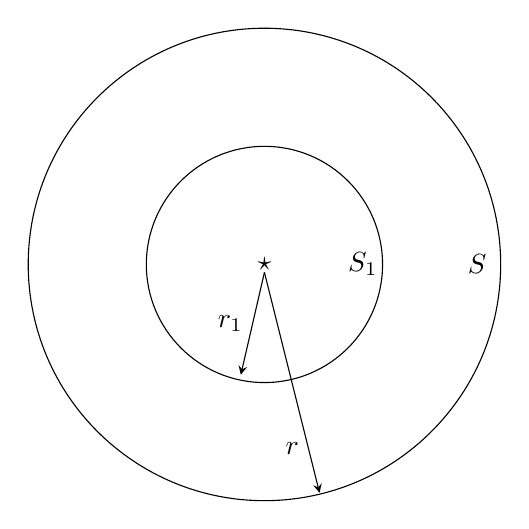
\begin{tikzpicture}
            \draw (0,0) circle (3);
            \draw (0,0) circle (1.5);
            \draw[-stealth] (0,-0.1) -- (-0.3,-1.4) node[left, pos=.5]{$r_1$};
            \draw[-stealth] (0,-0.1) -- (0.7,-2.9) node[left, pos=0.8]{$r$};
            \node(h1) at (1.25,0){$S_1$};
            \node(h2) at (2.7,0){$S$};
            \node(stella) at (0,0){$\star$};
        \end{tikzpicture}
    }
\end{wrapfigure}
 Un esempio è una stella sferica isolata. Ponendo due superfici immaginarie $S_1$ e $S$ con raggi $r_1$ e $r$, centrate nella stella, per la conservazione dell'energia sappiamo che l'energia ce passa attraverso $S_1$ è la stessa che passa attraverso $S$, quindi
\begin{gather*}
    F(r_1)\cdot 4\pi r_1^2\cdot dt = F(r)\cdot 4\pi r^2\cdot dt\\
    \Rightarrow F(r) = \frac{F(r_1)r_1^2}{r^2}.
\end{gather*}
Considerando $S_1$ fissa, abbiamo
\begin{equation*}
    F=\frac{\text{costante}}{r^2}.
\end{equation*}
Abbiamo quindi che il flusso di radiazione va come $1/r^2$.

%%%%%%%%%%%%%%%%%%%%%%%%%%%%%%%%%%%%%%%%%%%%%%%%%%%%%%%%%%%%%%%%%%%%%%%%%%%%%%%%%%%%%%%%%%%%%%%%%%%%%%%%%%%%%%%%%%%%%%%
\section{Intensità specifica}
Condisderiamo l'elemento di superficie $dA$, parte di una sorgente, orientato con $\hat{n}$ come in figura. 

\begin{figure}[h!]
        \centering
        \resizebox{0.5\columnwidth}{!}{
        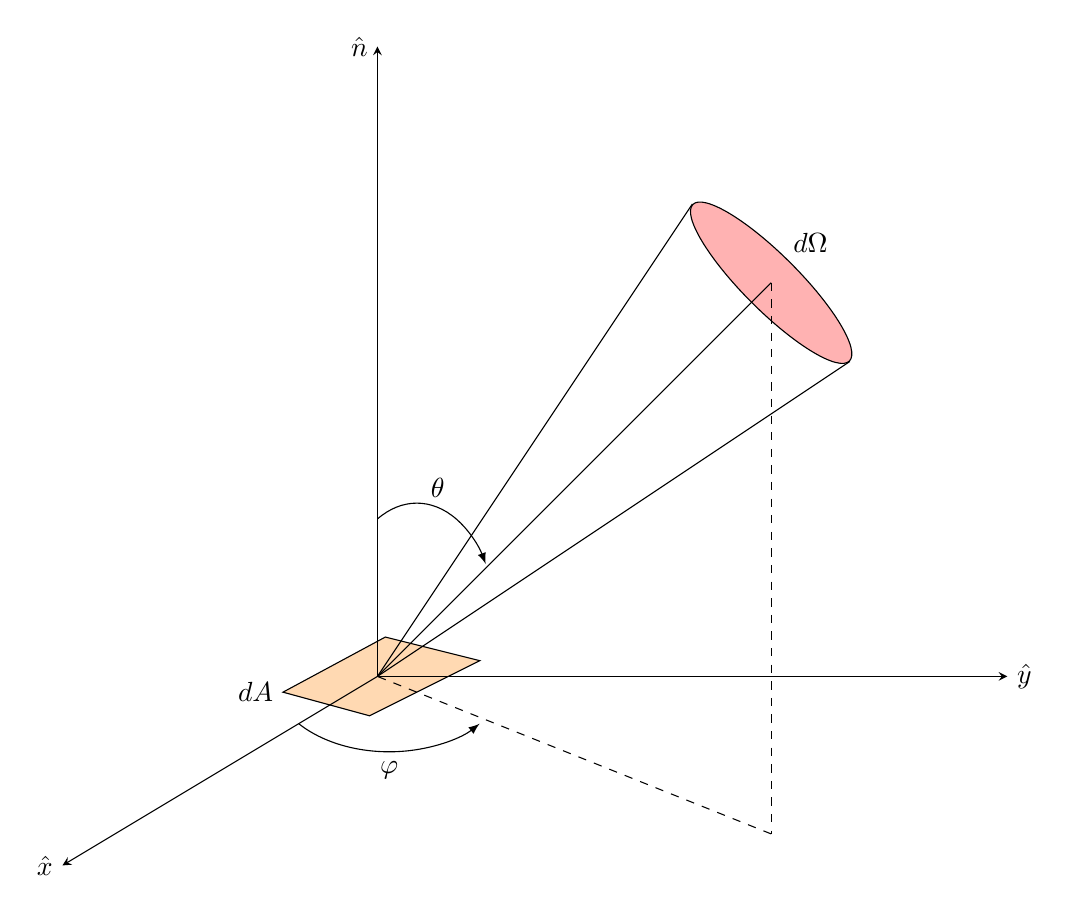
\begin{tikzpicture}
            \filldraw[fill=orange!30] (-1.2,-0.2) -- (0.1,0.5) -- (1.3,0.2) -- (-0.1, -0.5) -- cycle node[left, pos=1, color=black]{$dA$};
            \draw[-stealth] (0,0) -- (0, 8) node[left, pos=1]{$\hat{n}$};
            \draw[-stealth] (0,0) -- (8, 0) node[right, pos=1]{$\hat{y}$};
            \draw[-stealth] (0,0) -- (-4, -12/5) node[left, pos=1]{$\hat{x}$};
            \filldraw[rotate around={45:(5,5)},fill=red!30] (5,5) ellipse (10pt and 40pt);
            \node(ellips) at (5.5,5.5){$d\Omega$};
            \draw (0,0) -- (5,5);
            \draw (0,0) -- (6, 4);
            \draw (0,0) -- (4, 6);
            \draw[dashed] (5, 5) -- (5, -2);
            \draw[dashed] (5, -2) -- (0,0);
            \draw[-latex] (-1,-0.6) arc
                [
                    start angle=220,
                    end angle=320,
                    x radius=1.5cm,
                    y radius =1cm
                ] node[below, pos=0.5]{$\varphi$};
            \draw[-latex] (0,2) arc
                [
                    start angle=120,
                    end angle=29,
                    x radius=1cm,
                    y radius =1.5cm
                ] node[above, pos=0.5]{$\theta$} ;    
        \end{tikzpicture}
        }
\end{figure}
\noindent 
L'energia specifica (ad una certa frequenza) emessa in un tempo $dt$ da $dA$ nella banda $d\nu$ entro l'angolo solido $d\Omega$ è data da 
\begin{equation}
    dE_\nu \,d\nu=dE=\inu(\theta, \varphi)\cos\theta \,dA\,d\Omega \,d\nu\, dt
    \label{002}
\end{equation}
dove $\inu$ è detta intensità specifica (o radianza). Si misura in $\um{erg}\um{cm}^{-2}\um{s}^{-1}\um{ster}^{-1}\um{Hz}^-1$ o in $\um{W}\um{m}^{-2}\um{ster}^{-1}\um{Hz}^{-1}$.\\
$\inu$ dipende dalla posizione, dalla direzione e dalla frequenza. Nello stessa sistema della figura, il flusso a frequenza $\nu$ che passa dall'angolo solido $d\Omega$ (che quindi rispetto a \ref{001} riduce il flusso di un fattore $dA \cos\theta$) si scrive
\begin{equation*}
    dF_\nu=\inu \cos\theta\, d\Omega,
\end{equation*}
ed il flusso totale a frequenza $\nu$ sarà
\begin{equation*}
    F_\nu = \int \inu\cos\theta \,d\Omega,
\end{equation*}
che basterà integrare nelle frequenze per ottenere il flusso totale
\begin{equation*}
    F=\int F_\nu\, d\nu.
\end{equation*}
\paragraph{Nota:} Se $\inu$ fosse isotropa si avrebbe $F_\nu=0$ perché ci sarebbe uguale energia che attraversa con verso $\hat{n}$ e con verso $-\hat{n}$.\\
Per ottenere la quantità di moto per unità di area e di tempo (quindi la pressione) legata al flusso, normale rispetto a $dA$, basta ricordare che il momento del fotone è $p=E/c$, e di conseguenza il momento del flusso lungo un angolo $\theta$ sarà $F_\nu/c$. Per ottenere la componente lungo $\hat{n}$ basta moltiplicare per $\cos \theta$, così otteniamo
\begin{equation*}
    p_\nu = P_\nu = \frac{1}{c}\int\inu\cos^2\theta\, d\Omega
\end{equation*}

\section{Densità di energia radiativa}
Consideriamo l'energia in funzione della sua densità per unità di angolo solido
\begin{equation*}
    dE = u_\nu(\Omega)\,dV\,d\Omega\,d\nu.
\end{equation*}
Consideriamo un cilindro attorno ad un fascio con lunghezza $cdt$ e area $dA$.
\begin{figure}[h!]
        \centering
        \resizebox{0.5\columnwidth}{!}{
        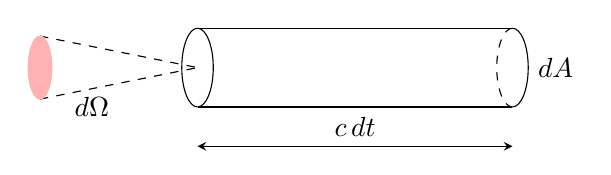
\begin{tikzpicture}
            \draw[dashed] (-1,0.9)--(1,0.5);
            \draw[dashed] (-1,0.1) -- (1,0.5);
            \filldraw[red!30] (-1,0.5) ellipse (0.15cm and 0.4cm) node[left, pos=0.5, black]{$d\Omega$};
            \draw (1,1) -- (5, 1);
            \draw (1,0) -- (5,0);
            \draw[stealth-stealth] (1, -0.5) -- (5, -0.5) node[above, pos=0.5]{$c\,dt$};
            \draw (1,1) arc
                [
                    start angle=90,
                    end angle=270,
                    x radius=0.2cm,
                    y radius =0.5cm
                ];
            \draw[dashed] (5,1) arc
                [
                    start angle=90,
                    end angle=270,
                    x radius=0.2cm,
                    y radius =0.5cm
                ];
            \draw (1,1) arc
                [
                    start angle=90,
                    end angle=-90,
                    x radius=0.2cm,
                    y radius =0.5cm
                ];
            \draw (5,1) arc
                [
                    start angle=90,
                    end angle=-90,
                    x radius=0.2cm,
                    y radius =0.5cm
                ] node[right, pos=0.5]{$dA$};
        \end{tikzpicture}
        }
\end{figure}
\\
Si ha che
\begin{equation*}
    dE=u_\nu(\Omega)\,dA\,c\,dt\,d\Omega\, d\nu.
\end{equation*}
Riscriviamo l'Eq. \ref{002} considerando $\theta=0$:
\begin{equation*}
    dE=\inu \,dA\,dt\,d\Omega\, d\nu.
\end{equation*}
Quindi ho che 
\begin{equation*}
    u_\nu(\Omega)=\frac{\inu}{c}.
\end{equation*}
Integrando nell'angolo solido si ottiene
\begin{equation}
    u_\nu = \frac{1}{c}\int\inu \,d\Omega = \frac{4\pi}{c}J_\nu,
    \label{003}
\end{equation}
in cui abbiamo definito l'intensità specifica media $J_\nu=\frac{1}{4\pi}\int\inu\, d\Omega$. \\
La densità di energia della radiazione totale si ottiene semplicemente integrando nella frequenza
\begin{equation*}
    u=\int u_\nu\,d\nu=\frac{4\pi}{c}\int J_\nu\,d\nu.
\end{equation*}
%%%%%%%%%%%%%%%%%%%%%%%%%%%%%%%%%%%%%%%%%%%%%%%%%%%%%%%%%%%
\section{Pressione di radiazione}
La pressione di radiazione su una superficie è data dal flusso del momento perpendicolare ad essa ($P=p/(dA\,dt)$). Come visto prima, il momento associato all'energia $dE_\nu$ vale $dE_\nu/c$ e a sua componente normale a $dA$ è $dE_\nu \cos\theta /c$. Dividendo per $dA\,dt$ otteniamo dalla \ref{002}
\begin{equation*}
    \frac{dE_\nu\,\cos\theta}{c\,dA\,dt}=\frac{\inu\cos^2\theta}{c}\,d\Omega.
\end{equation*}
Integrando in tutte le direzioni, la pressione di radiazione vale
\begin{equation*}
    P_\nu=\frac{1}{c}\int\inu\cos^2\theta\,d\Omega.
\end{equation*}
Se la radiazione è isotropa si ha
\begin{equation*}
    P_\nu=\frac{\inu}{c}\int\cos^2\theta\,d\Omega = \frac{4\pi}{3c}\inu\\
\end{equation*}
\paragraph{Nota:}
\begin{equation*}
    \int\cos^2\theta\,d\Omega=\int_0^{2\pi}\,d\varphi \int_0^\pi \cos^2\theta\sin\theta\,d\theta =2\pi\int_{1}^{-1}u^2(-du)=2\pi\left[\frac{u^3}{3}\right]_{1}^{-1}=\frac{4}{3}\pi
\end{equation*}
con $\cos\theta=u$ e $du=-\sin\theta\,d\theta$.\\
In caso di isotropia l'eq. \ref{003} diventa
\begin{equation*}
    u_\nu = \frac{\inu}{c}\int\,d\Omega = \frac{4\pi}{c}\inu,
\end{equation*}
Da cui otteniamo
\begin{equation*}
    P_\nu=\frac{u_\nu}{3}
\end{equation*}
per radiazione isotropa.
%%%%%%%%%%%%%%%%%%%%%%%%%%%%%%%%%%%%%%%%%%%%%%%%
\section{Costanza dell'intensità specifica lungo un raggio}
\begin{figure}[h!]
        \centering
        \resizebox{0.7\columnwidth}{!}{
        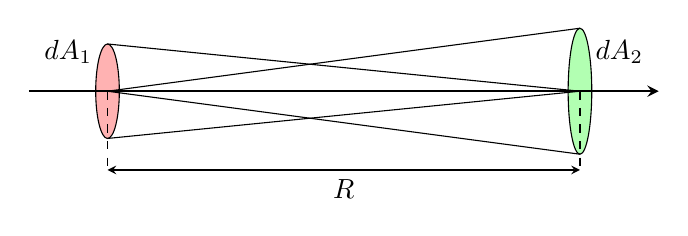
\begin{tikzpicture}
            \filldraw[fill=red!30] (-3,0.5) ellipse (0.15cm and 0.6cm);
            \filldraw[fill=green!30] (3,0.5) ellipse (0.15cm and 0.8cm);
            \draw[thin] (-3,1.1)--(3,0.5);
            \draw[thin] (-3,-0.1) -- (3,0.5);
            \draw[stealth-stealth] (-3, -0.5) -- (3, -0.5) node[below, pos=0.5]{$R$};
            \draw[thin] (-3,0.5)--(3,1.3);
            \draw[thin] (-3,0.5) -- (3,-0.3);
            \draw[thick,-stealth] (-4, 0.5) -- (4, 0.5);
            \draw[thin, dashed] (3,0.5) -- (3, -0.5);
            \draw[very thin, dashed] (-3,0.5) -- (-3, -0.5);
            \node at (-3.5,1) {$dA_1$};
            \node at (3.5,1) {$dA_2$};
        \end{tikzpicture}
        }
\end{figure}
Consideriamo due punti su un fascio e su ciascuno di essi costruiamo un'area, $dA_1$ e $dA_2$. Sfruttando la conservazione dell'energia scriviamo
\begin{equation*}
    dE_1 = I_{\nu_{1}}\,d\Omega_1\,dA_1\,d\nu_1\,dt_1 = dE_2 = I_{\nu_{2}}\,d\Omega_2\,dA_2\,d\nu_2\,dt_2.
\end{equation*}
$d\Omega_1$ è l'angolo solido sotteso da $dA_2$ a distanza $R$ dal punto in cui abbiamo costruito $dA_1$ e viceversa.\\
Dato che $d\Omega_1=dA_2/R^2$, $d\Omega_2=dA_1/R^2$, $d\nu_1=d\nu_2$ e $dt_1=dt_2$ si ha
\begin{gather*}
    I_{\nu_{1}}\,\frac{{dA_2}}{{R^2}}\,{dA_1}\,{d\nu\,dt} = I_{\nu_{2}}\,\frac{{dA_1}}{{R^2}}\,{dA_2}\,{d\nu\,dt}\\
    \Rightarrow I_{\nu_1} = I_{\nu_2} = I_\nu.
\end{gather*}
Quindi lungo un fascio, $\inu$ è costante.\\
Vogliamo mostrare che la costanza di $\inu$ e la legge dell'inverso del quadrato della distanza non sono in conflitto. Consideriamo la seguente situazione:
\begin{figure}[h!]
        \centering
        \resizebox{0.7\columnwidth}{!}{
        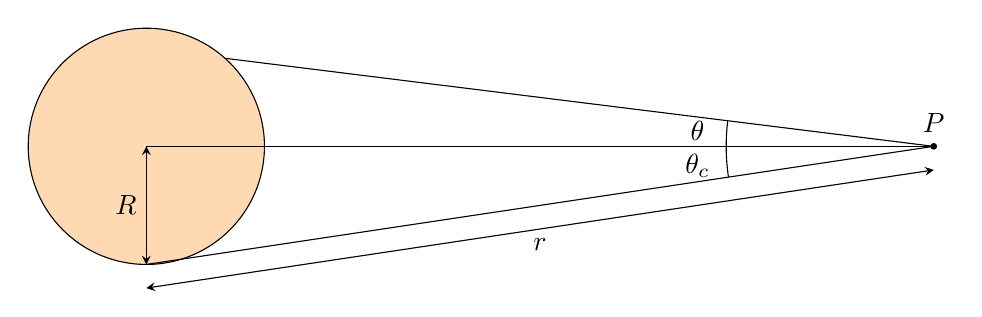
\begin{tikzpicture}
            \filldraw[fill=orange!30] (0,0) circle (1.5);
            \draw[stealth-stealth] (0, 0) -- (0, -1.5) node[left, pos=0.5]{$R$};
            \draw (0, 0) -- (10, 0);
            \filldraw [black] (10,0) circle (1pt);
            \draw (0,-1.5) -- (10,0); 
            \draw (1, 1.118) -- (10,0);
            \node at (10, 0.3) {$P$};
            \draw[stealth-stealth] ( 0, -1.8) -- (10,-0.3) node[below, pos=0.5]{$r$};
            \path[clip] (0,-1.5) -- (10,0) -- (0,1.24) -- cycle;
            \node[circle,draw=black,minimum size=150pt] at (10,0) (circ) {};
            \node at (7,-0.25) {$\theta_c$};
            \node at (7,0.2) {$\theta$};
        \end{tikzpicture}
        }
\end{figure}
calcoliamo il flusso di una stella che abbia intensità specifica uniforme $B$. \'E una sorgente isotropa, quindi al punto $P$ l'intensità sarà
\begin{equation*}
    I(P)=
    \begin{cases}
    B,\quad 0<\theta<\theta_c\\
    0,\quad \theta>\theta_c
    \end{cases}
\end{equation*}
con $\theta_c =\arcsin\frac{R}{r}$. Calcolando il flusso abbiamo
\begin{align*}
    F=\int I\cos\theta\,d\Omega &= B\int_{0}^{2\pi}\,d\varphi\int_{0}^{\theta_c}\cos\theta\sin\theta\,d\theta =\\
    &=2\pi B\int_{0}^{\cos\theta_c}-u\,du=\\
    &=\pi B(1-\cos^2\theta_c)=\\
    &=\pi B \sin^2\theta_c=\\
    &=\pi B \frac{R^2}{r}.
\end{align*}

\section{Trasporto radiativo}
Quando un fascio passa attraverso la materia, l'energia può essere fornita o sottratta per assorbimento ed emissione, ed in generale l'intensità specifica non resterà costante.
\subsection{Emissione}
Il coefficiente di emissione spontanea $j$ è definito come l'energia emessa per unità di tempo, per unità di angolo solido e per unità di volume
\begin{equation*}
    dE = j\,dt\,d\Omega\,dV.
\end{equation*}
Il coefficiente di emissione monocromatico si definisce analogamente
\begin{equation*}
    dE_\nu\, d\nu = dE = j_\nu\, dt\, d\Omega\,dV\,d\nu,
\end{equation*}
in cui $j_\nu$ ha le unità di $\um{erg}\um{s}^{-1}\um{ster}^{-1}\um{cm}^{-3}\um{Hz}^{-1}$.\\
Percorrendo una distanza $ds$, un fascio con sezione $dA$ attraversa un volume $dV=dA\,ds$. Quindi l'intensità aggiunta al fascio per emissione sèpntanea è
\begin{equation}
    d\inu = j_\nu\,ds.
    \label{004}
\end{equation}

\subsection{Assorbimento}
Definiamo il coefficiente di assorbimento, $\anu$ ($\um{cm}^{-1}$), con la seguente equazione, che rappresenta la perdita di intensità in un raggio che percorre una distanza $ds$
\begin{equation}
    d\inu=-\anu\inu\,ds
    \label{005}
\end{equation}
(per convenzione $\anu$ è positivo quando il raggio perde energia). Questa legge fenomenologica può essere compresa in termini di un modello microscopico in cui particelle con densità $n$ (numero di particelle per unità di volume) hanno ognuna una sezione d'urto $\snu$. Si assume che le particelle siano distribuite casualmente. Consideriamo gli effetti di questi assorbitori sulla radiazione attraverso $dA$ entro un angolo solido $d\Omega$.